\chapter{Background}

\section{Meta Pseudo-Labels}
Large models usually tend to overfit on 
small labeled datasets, and semi-supervised learning can help to mitigate this 
issue by leveraging the information contained in the unlabeled data.
However, to apply semi-supervised learning methods in practice, unlabeled data 
needs to carry useful information that is not already contained in the labeled 
dataset. This hypothesis can be formulated through three different assumptions: 
\emph{smoothness}, \emph{clusters}, and \emph{manifold} 
\cite{chapelle2010semi}.

\subsection{The Smoothness Assumption}
\textbf{Assumption}: If two examples are close in the input space, then they 
have similar outputs (labels).

The smoothness assumption implies that slightly changing the input data should 
not drastically change the output. Therefore, also the model is supposed to 
predict similar outputs for similar inputs. This assumption is fundamental in 
the propagation of the labels on the unlabelled data from the prior knowledge.

\subsection{The Cluster Assumption}
\textbf{Assumption}: Data points are orgnaized in clusters, and points that 
belong to the same cluster are more likely to have the same label.

This assumption supports methods like clustering followed by label propagation, 
where each cluster receives a common label, potentially inferred from a few 
labeled examples within or near the cluster.
It does not imply that each class is related to a unique cluster. 
On the other hand, it means that it is not possible to have two different classes 
in the same cluster.
From this hypothesis, it is also derived the \emph{low-density separation} 
assumption, which imposes that the decision boundary should lie in low-density
regions between clusters.

\begin{figure}[h]
    \centering
    \begin{minipage}{0.5\textwidth}
        \centering
        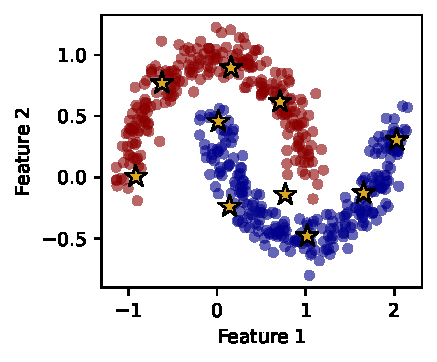
\includegraphics[height=6cm]{images/ssl/moon.pdf} % first figure
    \end{minipage}\hfill
    \begin{minipage}{0.44\textwidth}
        \centering
        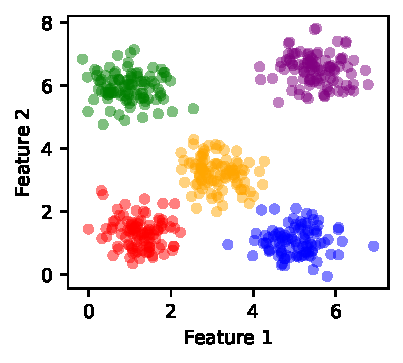
\includegraphics[height=6cm]{images/ssl/clusters.pdf} % second figure
    \end{minipage}
    \caption{Smoothness and cluster assumptions. \textbf{Left}: The moon dataset representing smoothness between 
        data points of each class. \textbf{Right}: The cluster assumption 
        illustrated with a toy example.}
    \end{figure}

\begin{figure}[h]
    \centering
    \begin{minipage}{0.4\textwidth}
        \centering
        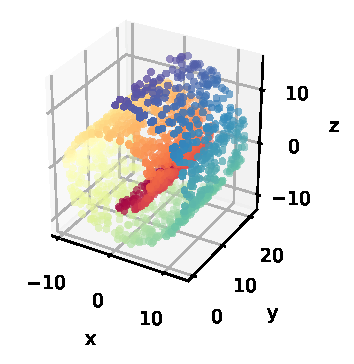
\includegraphics[height=6cm]{images/ssl/swiss_roll_3d.pdf} % first figure
    \end{minipage}\hfill
    \begin{minipage}{0.55\textwidth}
        \centering
        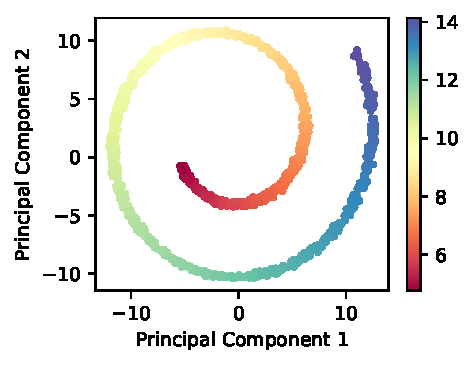
\includegraphics[height=6cm]{images/ssl/swiss_roll_pca.pdf} % second figure
    \end{minipage}
    \caption{Illustration of the manifold assumption. 
        \textbf{Left}: Data points are distributed in a high-dimensional space. 
        \textbf{Right}: The data points lie on a lower-dimensional manifold.}
\end{figure}

\subsection{The Manifold Assumption}
\textbf{Assumption}: The data lies on a low-dimensional manifold embedded in a 
high-dimensional space.

This assumption is based on the idea that the data is not distributed uniformly 
in the input space, but it is concentrated on a lower-dimensional manifold.
It is fundamental to avoid problems related to the curse of dimensionality, 
which can lead to overfitting and poor generalization because of sparse data.


\subsection{Problem Formulation}
In a more formal formulation, given $p(y|\bm{x}, D_L)$ as the probability 
distribution over the possible classes, given the input $x$ and the labeled 
dataset $D_L$, the goal is to estimate $p(y|\bm{x}, D_L, D_U)$, where $D_U$ is the 
unlabeled dataset. We can say that semi-supervised learning is effective only if 
$p(y|\bm{x}, D_L, D_U)$ is more accurate than $p(y|\bm{x}, D_L)$. If it is not 
the case, semi-supervised learning does not provide any additional benefit to 
the inference of the model, and it could even deteriorate the performance 
\cite{chapelle2010semi}.
